% Chương 3

\chapter{HUMAN ACTIVITY RECOGNITION} 

\label{Chapter3} 
Bài toán của chúng ta xây dựng đó là bài toán nhận dạng các hành động con người qua webcam hoặc video. Các hành động con người thì rất nhiều vì vậy trong bài viết này mình chỉ nhận dạng một vài hành động thường ngày qua con người. Thuật toán chúng tôi xử dụng trong bài này là CNN và mạng LSTM kết hợp với công cụ MediaPipe . Chúng tôi sẽ tiếp cận để xây dựng mô hình nhận biết theo 3 hướng :
\begin{itemize}
    \item Sử dụng công cụ MediaPipe và xây dựng mạng LSTM
    \item Xây dựng mô hình ConvLSTM
    \item Xây dựng mô hình LRCN
\end{itemize}

\section{Sử dụng công cụ MediaPipe và mạng LSTM}
    \begin{figure}[h!]
	\centering
	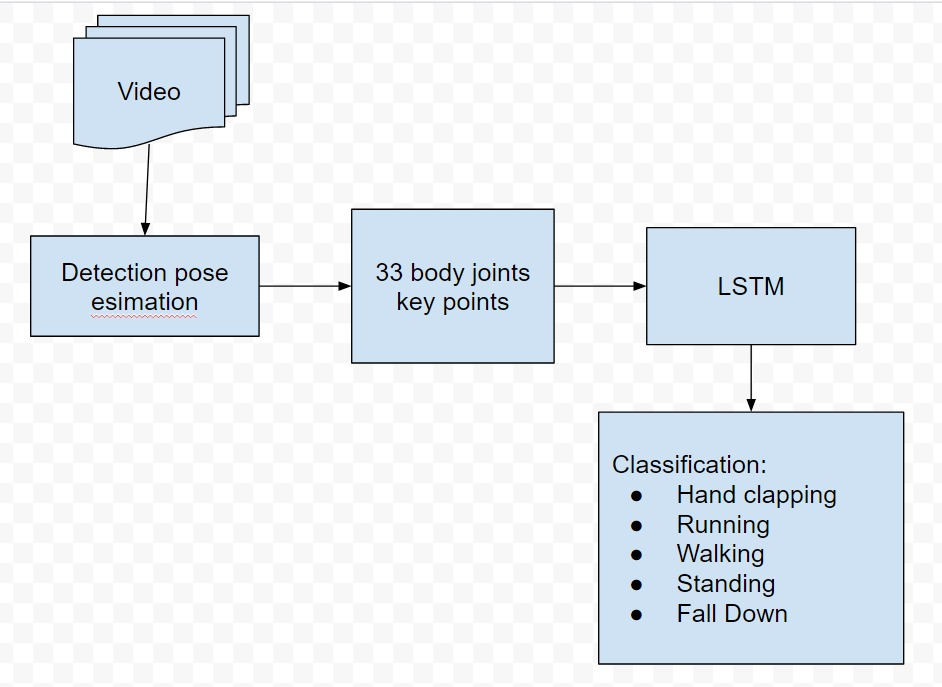
\includegraphics[width=0.7\textwidth]{Figures/luongbaitoan.jpeg}
	\caption[Luồng bài toán .]{Luồng bài toán.}
	\label{luongbaitoan.jpeg} 
    \end{figure}

\subsection{Tiền xử lý dữ liệu }
Tiền xử lý dữ liệu là một bước rất quan trọng trong việc giải quyết bất kỳ vấn đề nào trong lĩnh vực học máy. Hầu hết các bộ dữ liệu được sử dụng trong các vấn đề liên quan đến học máy cần được xử lý, làm sạch và biến đổi trước khi một thuật toán có thể được huấn luyện trên những bộ dữ liệu này.
\subsubsection{Thu thập dữ liệu }

    \begin{figure}[h!]
	\centering
	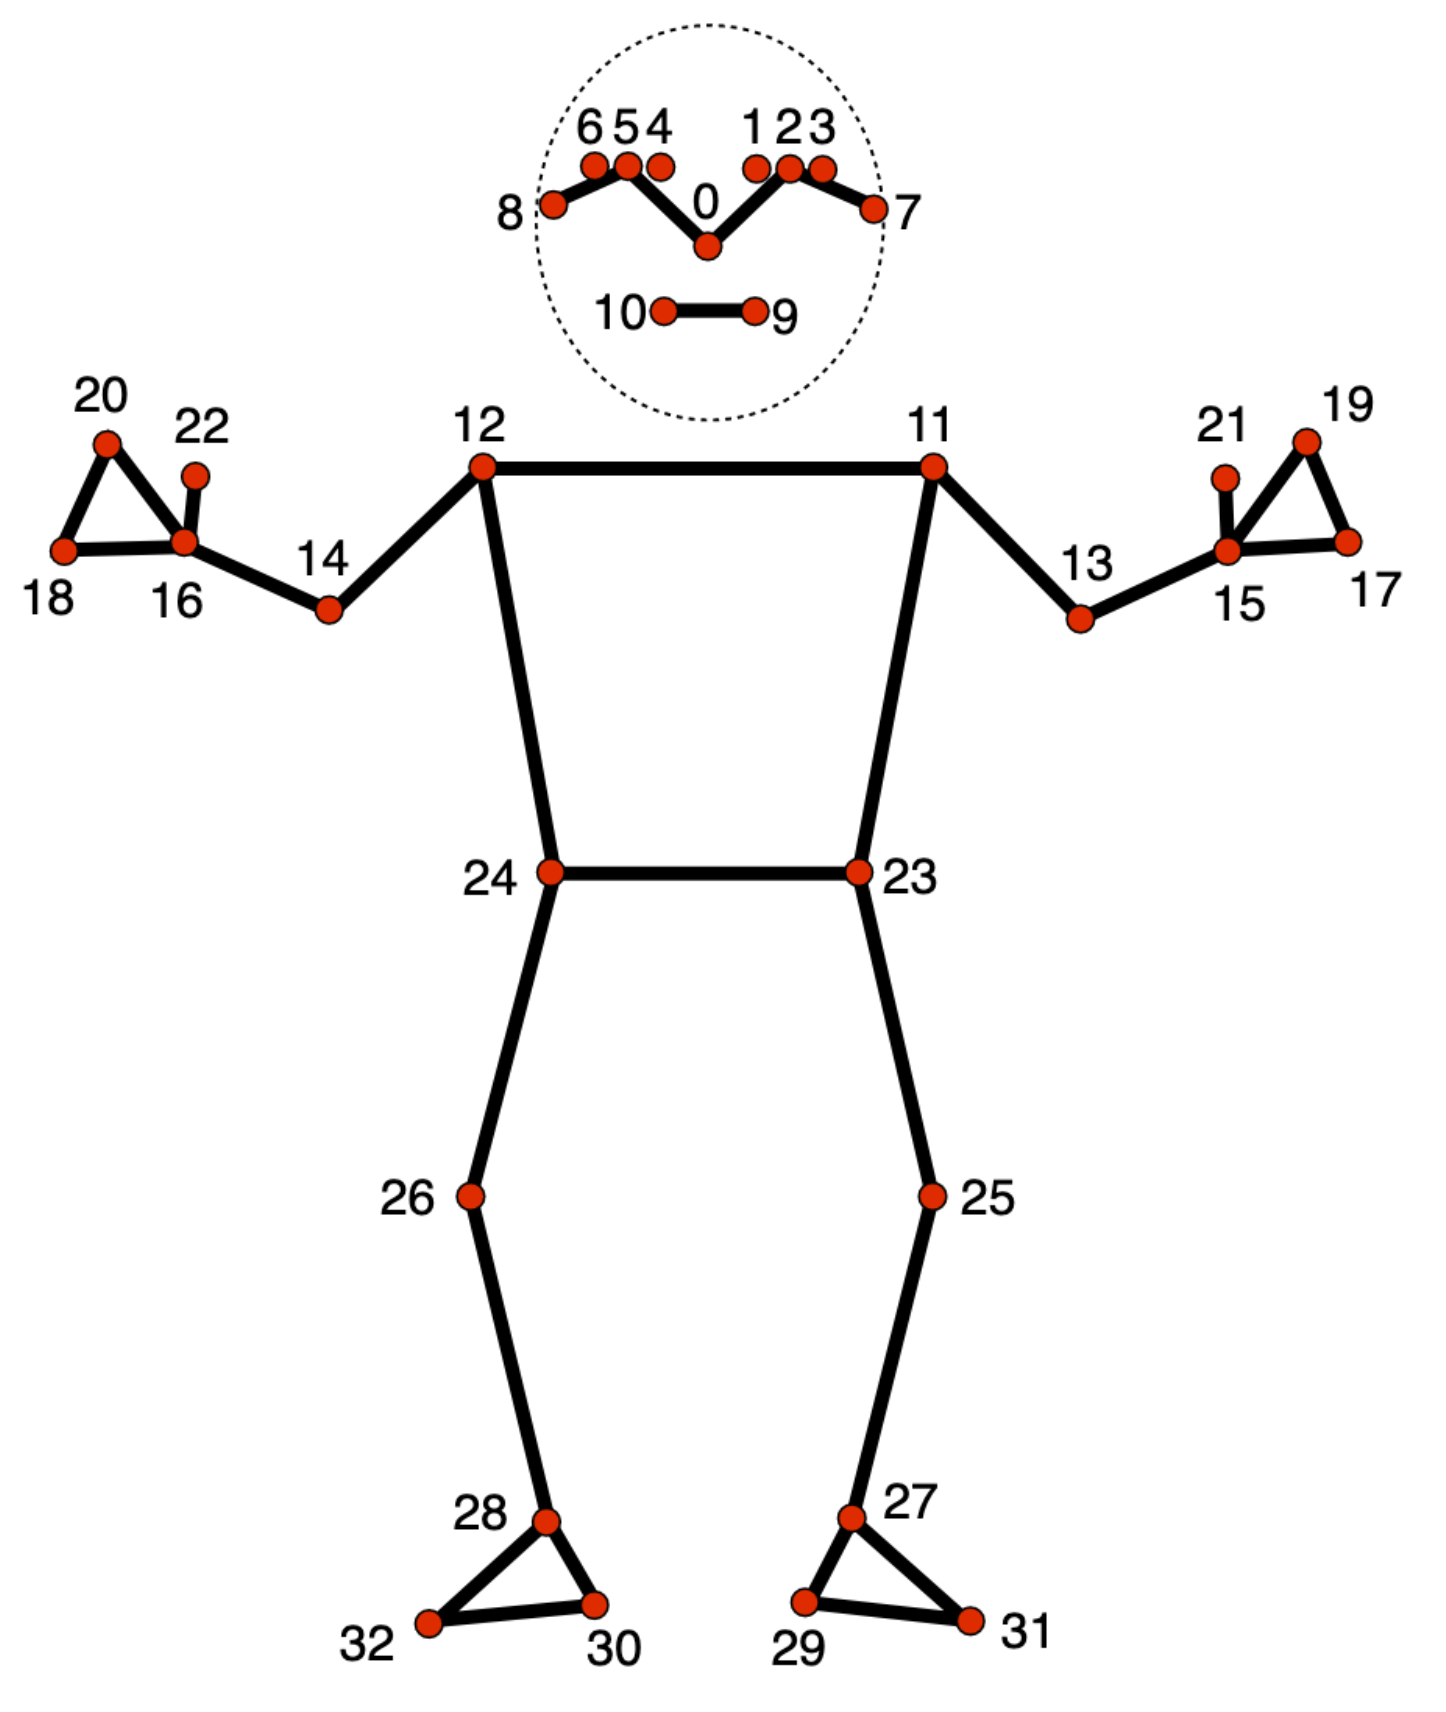
\includegraphics[width=0.7\textwidth]{Figures/pose_landmarks_index.png}
	\caption[MediaPipe Pose .]{MediaPipe Pose .}
	\label{pose_landmarks_index.png} 
    \end{figure}
Trước khi chuẩn bị dữ liệu cho đầu vào tôi sẽ giới thiệu về một công cụ mạnh mẽ \href{https://developers.google.com/mediapipe/solutions/vision/pose_landmarker/}{MediaPipe Pose} Mediapipe Pose để biết cách vẽ các điểm keypoints và cách hoạt động của nó như thế nào . Mỗi vị trí trong 33 keypoints đó đều có 4 điểm tương ứng hoặc có thể nói là tọa độ tương ứng đó là: X,Y,Z,VISIBILITY. Phần này chính là input của mạng LSTM. Chúng ta sẽ đưa 4 điểm tương ứng này với từng điểm keypoints(có 33 điểm) sẽ tao thành array, sau đó chúng ta làm phẳng nó ra 33*4 sẽ là 132 điểm. Thêm 1 vấn đề nữa là nếu như trong 1 khung hình mà không thể hết được 33 điểm thì các vị trí không thể vẽ được được gán bằng 0 hoặc xấp xỉ không nếu không nhìn rõ . 
Đầu tiên cần khởi tạo thư viện mediapipe . 

\begin{lstlisting}[style=codePython]
 	import cv2
import mediapipe as mp
import pandas as pd

cap = cv2.VideoCapture(0)

mpPose = mp.solutions.pose
pose = mpPose.Pose()
mpDraw = mp.solutions.drawing_utils
\end{lstlisting}

Bây giờ sử dụng thư viện để tìm các điểm , vẽ điểm nút và sau đó vẽ đường nối các điểm nút lại . Ghi lại các thông số data vào list . Sử dụng thư viện pandas để lưu dữ liệu thu được vao file txt 
\begin{lstlisting}[style=codePython]
lm_list = []
label = "CLAP"
no_of_frames = 600

def make_landmark_timestep(results):
    print(results.pose_landmarks.landmark)
    c_lm = []
    for id, lm in enumerate(results.pose_landmarks.landmark):
        c_lm.append(lm.x)
        c_lm.append(lm.y)
        c_lm.append(lm.z)
        c_lm.append(lm.visibility)
    return c_lm

def draw_landmark_on_image(mpDraw, results, img):
    mpDraw.draw_landmarks(img, results.pose_landmarks, mpPose.POSE_CONNECTIONS)

    for id, lm in enumerate(results.pose_landmarks.landmark):
        h, w, c = img.shape
        print(id, lm)
        cx, cy = int(lm.x * w), int(lm.y * h)
        cv2.circle(img, (cx, cy), 10, (0, 0, 255), cv2.FILLED)
    return img


while len(lm_list) <= no_of_frames:
    ret, frame = cap.read()
    if ret:
        frameRGB = cv2.cvtColor(frame, cv2.COLOR_BGR2RGB)
        results = pose.process(frameRGB)

        if results.pose_landmarks:
            lm = make_landmark_timestep(results)
            lm_list.append(lm)
            frame = draw_landmark_on_image(mpDraw, results, frame)

        cv2.imshow("image", frame)
        if cv2.waitKey(1) == ord('q'):
            break

df  = pd.DataFrame(lm_list)
df.to_csv(label + ".txt")
cap.release()
cv2.destroyAllWindows()
\end{lstlisting}

\subsubsection{Chuẩn hóa dữ liệu}
Trong học máy , chuẩn hóa dữ liệu là một bước rất quan trọng dường như là không thể thiếu trong việc xây dựng mô hình .Việc chuẩn hóa dữ liệu sẽ giúp cho mô hình đạt được kết quả tốt . Trong phần này nhóm sẽ trình bày phương pháp nhóm sử dụng để chuẩn hóa dữ liệu . Đầu tiên sử dụng thư viện pandas để đọc dữ liệu thu được 
\begin{lstlisting}[style=codePython]
import numpy as np
import pandas as pd

from keras.layers import LSTM, Dense, Dropout, BatchNormalization
from keras.models import Sequential
from keras.utils import to_categorical

from sklearn.model_selection import train_test_split

bodyswing_df = pd.read_csv("../data/SWING.txt")
handswing_df = pd.read_csv("../data/HANDSWING.txt")
doze_df = pd.read_csv("../data/DOZE.txt")
love_df = pd.read_csv("../data/LOVE.txt")
clap_df = pd.read_csv("../data/CLAP.txt")
X = []
y = []
no_of_timesteps = 10

dataset_body = bodyswing_df.iloc[:,1:].values
n_sample = len(dataset_body)
for i in range(no_of_timesteps, n_sample):
    X.append(dataset_body[i-no_of_timesteps:i,:])
    y.append(0)

dataset_hand = handswing_df.iloc[:,1:].values
n_sample = len(dataset_hand)
for i in range(no_of_timesteps, n_sample):
    X.append(dataset_hand[i-no_of_timesteps:i,:])
    y.append(1)


dataset_doze = doze_df.iloc[:,1:].values
n_sample = len(dataset_doze)
for i in range(no_of_timesteps, n_sample):
    X.append(dataset_doze[i-no_of_timesteps:i,:])
    y.append(2)

dataset_love = love_df.iloc[:,1:].values
n_sample = len(dataset_love)
for i in range(no_of_timesteps, n_sample):
    X.append(dataset_love[i-no_of_timesteps:i,:])
    y.append(3)

dataset_clap = clap_df.iloc[:,1:].values
n_sample = len(dataset_clap)
for i in range(no_of_timesteps, n_sample):
    X.append(dataset_clap[i-no_of_timesteps:i,:])
    y.append(4)
\end{lstlisting}

Dữ liệu trong file CSV sẽ được load bằng thư viện pandas. Đối với dữ liệu đầu vào nhóm chia ra thành các lô gồm 10 dữ liệu với mỗi dữ liệu là 1 lần lấy được các điểm , mỗi lần sẽ lấy được 132 giá trị  . 

\begin{lstlisting}[style=codePython]
    X, y = np.array(X), np.array(y)

print(X.shape, y.shape)

X_train, X_test, y_train, y_test = train_test_split(X, y, test_size=0.2)
# 132 = 4 * 33
# 10 = no_of_number


# one hot encoding

y_train_onehot = to_categorical(y_train)
y_test_onehot = to_categorical(y_test)
print(y_train_onehot.shape , y_test_onehot.shape)
n_features = X.shape[2]
\end{lstlisting}

Do mô hình là mô hình phân loại nhiều lớp nên các hành động sẽ phải được one hot encode bằng hàm one\_hot\_encode() như trên.

Dữ liệu được chia thành tập train và tập test: Sau đó ta tạo 4 biến, gồm X$\_$train, y$\_$train và X$\_$test, y$\_$test. Với đối số truyền vào là giá trị X, y ta đã lấy từ dữ liệu bên trên, test$\_$size trả về cho ta phần trăm dữ liệu được chia, ví dụ 0.2 tương ứng với dữ liệu được chia thành 20\% giá trị là test, còn lại là dữ liệu train. random$\_$state bằng một số tương ứng nào đó để đảm bảo mỗi lần ta chạy lại mô hình, giá trị phân tách ngẫu nhiên nhận được là giống nhau, bạn có thể cho số nào bất kỳ.  


\section{Xây dựng mô hình}

\begin{lstlisting}[style=codePython]
    model = Sequential()
    model.add(LSTM(128, return_sequences=True, activation='relu', input_shape=(no_of_timesteps, n_features)))
    model.add(Dropout(0.2))
    model.add(LSTM(256, return_sequences=True, activation='relu'))
    model.add(Dropout(0.2))
    model.add(LSTM(256, return_sequences=False, activation='relu'))
    model.add(BatchNormalization())
    model.add(Dense(256, activation='relu'))
    model.add(Dense(128, activation='relu'))
    model.add(Dense(64, activation='relu'))
    model.add(Dense(5, activation='softmax'))
    
    model.compile(optimizer="adam", metrics = ['accuracy'], loss = "categorical_crossentropy")
    model.fit(X_train, y_train_onehot, epochs=20, batch_size=32,validation_data=(X_test, y_test_onehot))
    model.save("model_16.h5")
\end{lstlisting}
Đối với mô hình LSTM, dữ liệu sẽ được reshape lại thành dạng (samples, no\_of\_timesteps, features) với samples là số lượng mẫu, time steps là số lượng data liền trước và features là số lượng đặc trưng của mỗi mẫu .
Mô hình được xây dựng bởi 3 lớp LSTM và 4 lớp kết nối đầy đủ. Thư viện tensorflow cung cấp đầy đủ chức năng cần thiết để xây dựng mô hình như trên. Ở đây hai lớp LSTM đầu tiên sẽ đặt tham số 'return\_sequences=True' để cho phép LSTM layer sẽ trả về chuỗi kết quả cho mỗi bước thời gian trong chuỗi đầu vào.
\begin{itemize}
	\item Thêm một lớp LSTM với 128 đơn vị, trả về các chuỗi, sử dụng hàm kích hoạt ReLU và chỉ định hình dạng đầu vào.
	\item Sau mỗi lớp LSTM, Thêm một lớp dropout với tỷ lệ dropout là 0.2
	\item Thêm một lớp LSTM khác với 256 đơn vị, trả về các chuỗi, sử dụng hàm kích hoạt ReLU.
        \item Thêm một lớp LSTM khác với 256 đơn vị, không trả về chuỗi, sử dụng hàm kích hoạt ReLU.
	\item Thêm một lớp chuẩn hóa theo batch.
        \item Thêm các lớp kết nối đầy đủ với hàm kích hoạt ReLU.
        \item Cuối cùng là 1 lớp kết nối đầy đủ với hàm kích hoạt softmax
\end{itemize}
Sau khi xây dựng mô hình, mô hình sẽ được biên dịch với hàm mất mát là categorical\_crossentropy và hàm tối ưu hóa là adam. Sau đó, mô hình sẽ được huấn luyện với 20 epochs và batch size là 32.

*** Sau khi đã xây dựng được kiến trúc của mô hình . Bước tiếp theo là thực hiện huấn luyện mô hình

\subsection{Tiêu chí ảnh hưởng đến mô hình}	

Có nhiều yếu tố ảnh hưởng đến độ hiệu quả của một mô hình máy học. Dưới đây là một số tiêu chí quan trọng:

\begin{itemize}
	\item Độ rõ ràng và độ phong phú của dữ liệu: Mô hình sẽ hoạt động tốt hơn khi dữ liệu huấn luyện rõ ràng, có độ phân loại cao và đủ đa dạng. Dữ liệu không rõ ràng, nhiễu và thiếu thông tin có thể làm giảm độ hiệu quả của mô hình.
	
	\item Số lượng và chất lượng dữ liệu: Một số lượng dữ liệu huấn luyện đủ lớn có thể giúp mô hình học được các mẫu và mối quan hệ phức tạp. Đồng thời, chất lượng dữ liệu cũng quan trọng, bao gồm độ chính xác, đồng nhất và đại diện cho phân phối dữ liệu thực tế.
	
	\item Chọn mô hình phù hợp: Một mô hình phải được lựa chọn dựa trên yêu cầu cụ thể của bài toán. Mô hình phải có khả năng học và biểu diễn các mẫu và quan hệ trong dữ liệu một cách hiệu quả.
	
	\item Quá trình huấn luyện: Thời gian huấn luyện, tỷ lệ học tập, thuật toán tối ưu hóa và các siêu tham số khác cũng có thể ảnh hưởng đến hiệu quả của mô hình. Quá trình huấn luyện phải được điều chỉnh và tối ưu để đạt được kết quả tốt.
	
	\item Tính diễn giải và khả năng áp dụng: Một mô hình có khả năng diễn giải tốt và có thể áp dụng vào thực tế sẽ có hiệu quả cao hơn. Sự diễn giải giúp người dùng hiểu rõ quyết định của mô hình và tin tưởng vào kết quả dự đoán.	
\end{itemize}

\subsection{Tiêu chí đánh giá mô hình}

Khi đánh giá huấn luyện một mô hình máy học, có một số tiêu chí quan trọng cần xem xét. Dưới đây là một số tiêu chí phổ biến để đánh giá mô hình:

\begin{itemize}
	\item Độ chính xác (Accuracy): Đây là tiêu chí cơ bản để đánh giá khả năng dự đoán chính xác của mô hình trên tập dữ liệu kiểm tra. Độ chính xác được tính bằng tỷ lệ giữa số lượng dự đoán đúng và tổng số mẫu trong tập kiểm tra.
	
	\item Mất mát (Loss): Mất mát đo lường mức độ sai khác giữa các dự đoán của mô hình và giá trị thực tế tương ứng. Một hàm mất mát được sử dụng để đo lường sự sai khác này và mục tiêu là tìm cách giảm mất mát trong quá trình huấn luyện.
	
	\item Đồng nhất (Consistency): Mô hình cần cho ra kết quả tương tự khi được huấn luyện lại trên các tập dữ liệu khác nhau hoặc khi được huấn luyện nhiều lần trên cùng một tập dữ liệu. Sự đồng nhất giúp đảm bảo tính ổn định và tin cậy của mô hình.
	
	\item Quá khớp (Overfitting) và thiếu khớp (Underfitting): Quá khớp xảy ra khi mô hình đã học nhớ quá mức từ dữ liệu huấn luyện, nhưng không thể tổng quát hóa tốt cho các dữ liệu mới. Thiếu khớp xảy ra khi mô hình không học được đủ thông tin từ dữ liệu huấn luyện và không thể dự đoán chính xác trên dữ liệu mới. Đánh giá sự quá khớp và thiếu khớp là một tiêu chí quan trọng để đảm bảo mô hình có khả năng tổng quát hóa tốt.
	
	\item Thời gian huấn luyện (Training time): Thời gian huấn luyện là thời gian mô hình cần để học từ dữ liệu huấn luyện. Đánh giá thời gian huấn luyện là quan trọng đặc biệt khi xem xét các mô hình phức tạp hoặc dữ liệu lớn.	
	
	\item Khả năng diễn giải (Interpretability): Khả năng diễn giải của mô hình đo lường khả năng hiểu được lý do tại sao một dự đoán được thực hiện. Một mô hình diễn giải tốt có thể cung cấp giải thích rõ ràng và logic cho quá trình ra quyết định.
	
	\item Hiệu suất tính toán (Computational performance): Đánh giá hiệu suất tính toán của mô hình là quan trọng, đặc biệt khi triển khai mô hình trên các hệ thống có tài nguyên hạn chế. Thời gian dự đoán và khả năng làm việc với dữ liệu lớn là những yếu tố quan trọng để xem xét.
\end{itemize}

$\Longrightarrow$ Những tiêu chí trên là chỉ một số ví dụ phổ biến. Đánh giá mô hình cần tuân thủ các tiêu chí phù hợp với bài toán cụ thể và ngữ cảnh sử dụng mô hình đó.



\subsubsection{Kết quả huất luyện mô hình}

\begin{figure}[h!] 
	\begin{tabular}{cc}
		\centering
		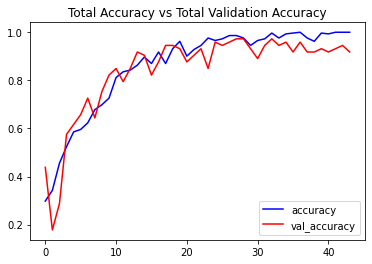
\includegraphics[width=0.5\textwidth]{Figures/acc_model1.png} &
		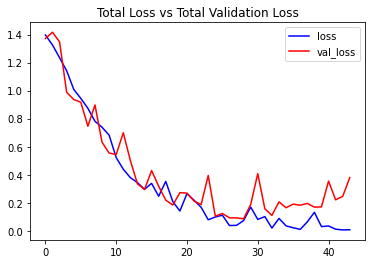
\includegraphics[width=0.5\textwidth]{Figures/loss_model1.png} 
	\end{tabular}
	\caption[Model Accuracy và Model Loss.]{Model Accuracy và Model Loss.}
	\label{fig:modelloss_and_Model Accuracy}
\end{figure}

Đồ thị ACC,  độ chính xác (Accuracy) lên đến 98\% và bắt đầu ổn định khi epoch = 20,  cho cả tập dữ liệu huấn luyện và tập test, đồ thị Loss của cũng cho thấy sau mức này, Loss của cả tập train và validation. Kết quả cho thấy mô hình có độ phù hợp tốt và không bị quá khớp (over-fitting).

\begin{itemize}
	\item Đánh giá hiệu suất mô hình:
	
	\begin{figure}[h!]
		\centering
		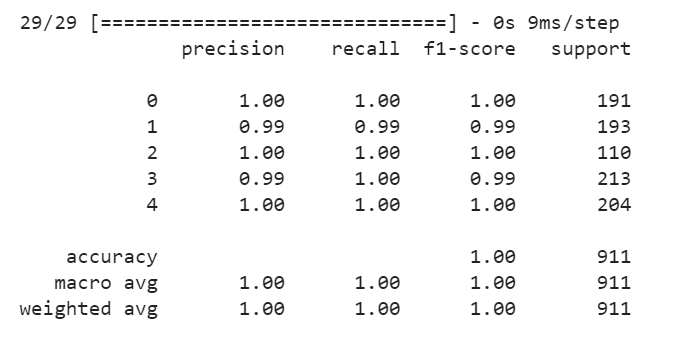
\includegraphics[width=0.7\textwidth]{Figures/evaluate_model1.PNG}
		\caption[Đánh giá hiệu suất mô hình.]{Đánh giá hiệu suất mô hình.}
		\label{fig:ac} 
	\end{figure}
	
	\item Confusion Matrix:
	
	\begin{figure}[h!]
		\centering
		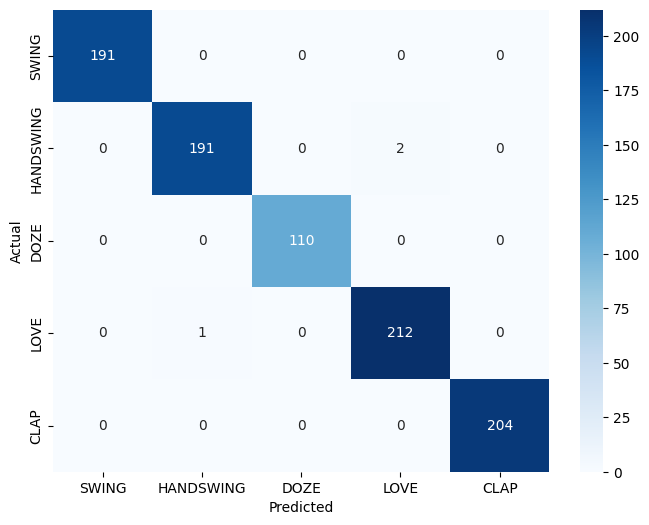
\includegraphics[width=0.6\textwidth]{Figures/model1_confusion.png}
		\caption[Confusion Matrix.]{Confusion Matrix.}
		\label{fig:fu} 
	\end{figure}
\end{itemize}

\subsection{Thử nghiệm với thời gian thực webcam}

*** Sử dụng thư viện open cv để test kết quả trên thời gian thực 

** Bước 1: Import thư viện và Load Model

\begin{lstlisting}[style=codePython]
import cv2
import mediapipe as mp
import numpy as np
import threading
import tensorflow as tf

label = "Warmup...."
n_time_steps = 10
lm_list = []

mpPose = mp.solutions.pose
pose = mpPose.Pose()
mpDraw = mp.solutions.drawing_utils

model = tf.keras.models.load_model("model_19.h5")					
\end{lstlisting}

** Bước 2: Các hàm phụ trợ vẽ điểm nút nối các điểm nút và hàm dự đoán kết quả

\begin{lstlisting}[style=codePython]
def make_landmark_timestep(results):
    c_lm = []
    for id, lm in enumerate(results.pose_landmarks.landmark):
        c_lm.append(lm.x)
        c_lm.append(lm.y)
        c_lm.append(lm.z)
        c_lm.append(lm.visibility)
    return c_lm


def draw_landmark_on_image(mpDraw, results, img):
    mpDraw.draw_landmarks(img, results.pose_landmarks, mpPose.POSE_CONNECTIONS)
    for id, lm in enumerate(results.pose_landmarks.landmark):
        h, w, c = img.shape
        # print(id, lm)
        cx, cy = int(lm.x * w), int(lm.y * h)
        cv2.circle(img, (cx, cy), 5, (255, 0, 0), cv2.FILLED)
    return img


def draw_class_on_image(label, img):
    font = cv2.FONT_HERSHEY_SIMPLEX
    bottomLeftCornerOfText = (10, 30)
    fontScale = 1
    fontColor = (0, 255, 0)
    thickness = 2
    lineType = 2
    cv2.putText(img, label,
                bottomLeftCornerOfText,
                font,
                fontScale,
                fontColor,
                thickness,
                lineType)
    return img


def detect(model, lm_list):
    global label
    lm_list = np.array(lm_list)
    lm_list = np.expand_dims(lm_list, axis=0)
    print(lm_list.shape)

    y_hat = model.predict(lm_list)
    results = np.argmax(y_hat)
    print(y_hat , results)


    label_predict = ('body','hand','doze','love','clap')
    label = label_predict[results]
    return label
\end{lstlisting}

** Bước 3: Chạy webcam

\begin{lstlisting}[style=codePython]
while True:

    success, img = cap.read()
    imgRGB = cv2.cvtColor(img, cv2.COLOR_BGR2RGB)
    results = pose.process(imgRGB)
    i = i + 1
    if i > warmup_frames:
        print("Start detect....")

        if results.pose_landmarks:
            c_lm = make_landmark_timestep(results)

            lm_list.append(c_lm)
            if len(lm_list) == n_time_steps:
                # predict
                t1 = threading.Thread(target=detect, args=(model, lm_list))
                t1.start()
                #t1 = detect(model,lm_list)
                lm_list = []


            img = draw_landmark_on_image(mpDraw, results, img)

    img = draw_class_on_image(label, img)
    cv2.imshow("Image", img)
    if cv2.waitKey(1) == ord('q'):
        break

cap.release()
cv2.destroyAllWindows()							
\end{lstlisting}


\newpage

\section{Xây dựng mô hình sử dụng\href{https://keras.io/api/layers/recurrent_layers/conv_lstm2d/}{ConvLSTM2D layer} và mô hình LRCN}
\subsection{Tiền xử lý dữ liệu}


\subsubsection{Thu thập dữ liệu }

    Trong bài này nhóm xử dụng bộ dự liệu \href{https://www.crcv.ucf.edu/data/UCF50.php}{UCF50 - Action Recognition Dataset}
Bộ dữ liệu Nhận diện hành động, bao gồm các video thực tế được lấy từ YouTube, điều này làm cho bộ dữ liệu này khác biệt so với hầu hết các bộ dữ liệu nhận diện hành động khác vì chúng không phải là thực tế và được đóng bởi diễn viên. Bộ dữ liệu chứa :

\begin{itemize}
    \item 50 Danh mục hành động
    \item 133 Số video trung bình mỗi hành động
    \item 26 Số khung hình trung bình mỗi video
\end{itemize}


\begin{figure}[h!]
	\centering
	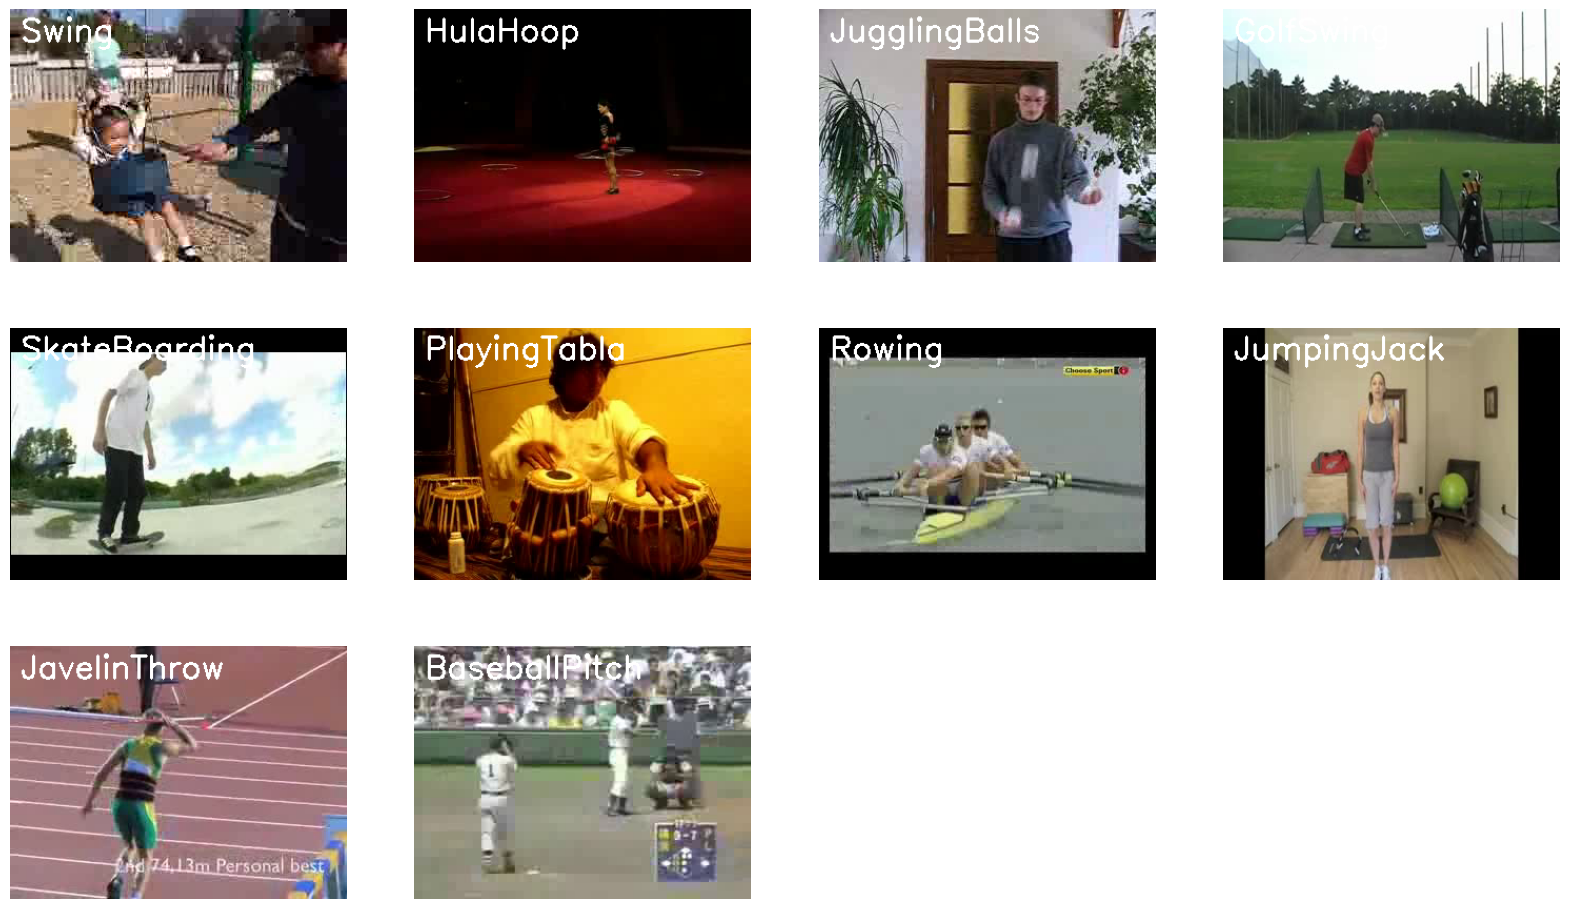
\includegraphics[width=0.7\textwidth]{Figures/datashow.png}
	\caption[Visualize the Data with its Labels.]{Visualize the Data with its Labels .}
	\label{datashow.png} 
    \end{figure}
    \newpage
\subsubsection{Tăng cường dữ liệu}
\begin{figure}[h!]
	\centering
	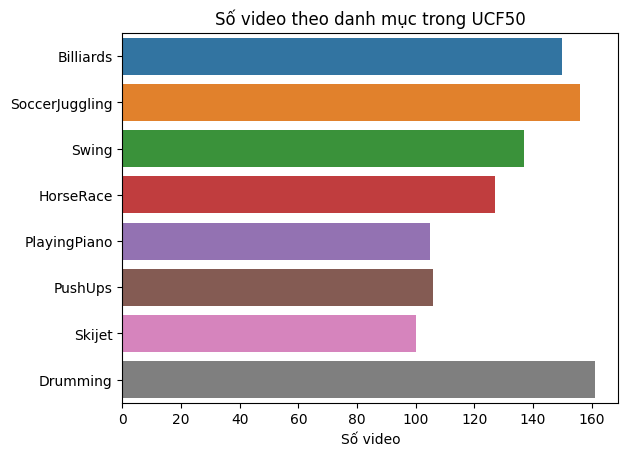
\includegraphics[width=0.7\textwidth]{Figures/numbersvideo.png}
	\caption[Visualize the numbers.]{Visualize the numbers .}
	\label{numbersvideo.png} 
    \end{figure}

Nhận thấy bộ dữ liệu này có sự chênh lệnh về dự liệu cũng như đây là bộ dữ liệu đã có từ 5 năm trước . Hiện nay video đã cải thiện chất lượng hơn . Nhóm đã thêm video tải từ youtube vào để dữ liệu cân bằng cũng như video có độ phân giải tốt hơn để khả năng dự đoán được cải thiện 

Sau khi tăng cường dataset mới được lưu trên drive : \href{https://drive.google.com/drive/folders/1GXIWkXE2PQTgVSl-xattG6JVyaDb1jgR?usp=sharing}{Dataset}
\subsubsection{Chuẩn hóa dữ liệu}
Đầu tiên, chúng ta sẽ đọc các tệp video từ bộ dữ liệu và thay đổi kích thước các khung hình của video thành chiều rộng và chiều cao cố định, để giảm thiểu tính toán và chuẩn hóa dữ liệu về khoảng [0-1] bằng cách chia giá trị pixel cho 255, điều này làm cho quá trình hội tụ nhanh hơn khi huấn luyện mạng.

Nhưng trước hết, hãy khởi tạo một số hằng số.


\begin{lstlisting}[style=codePython]
IMAGE_HEIGHT , IMAGE_WIDTH = 64, 64

SEQUENCE_LENGTH = 10

DATASET_DIR = "UCF50"
\end{lstlisting}

 Tiếp theo tạo một hàm frames\_extraction() sẽ tạo một danh sách chứa các khung hình đã thay đổi kích thước và chuẩn hóa của một video, đường dẫn của video sẽ được truyền vào hàm như một đối số. Hàm sẽ đọc tệp video từng khung hình một, mặc dù không phải tất cả các khung hình được thêm vào danh sách vì chúng ta chỉ cần một chuỗi độ dài khung hình phân phối đều. 

\begin{lstlisting}[style=codePython]
def frames_extraction(video_path):

    frames_list = []
    video_reader = cv2.VideoCapture(video_path)
    video_frames_count =int(video_reader.get(cv2.CAP_PROP_FRAME_COUNT))
    skip_frames_window = max(int(video_frames_count/SEQUENCE_LENGTH), 1)

    for frame_counter in range(SEQUENCE_LENGTH):

        video_reader.set(cv2.CAP_PROP_POS_FRAMES, frame_counter * skip_frames_window)
        
        success, frame = video_reader.read()
        if not success:
            break

        resized_frame = cv2.resize(frame, (IMAGE_HEIGHT, IMAGE_WIDTH))
        normalized_frame = resized_frame / 255
        frames_list.append(normalized_frame)
    video_reader.release()

    return frames_list
\end{lstlisting}

Bây giờ chúng ta sẽ tạo một hàm create\_dataset() sẽ lặp qua tất cả các lớp được chỉ định trong hằng số CLASSES\_LIST và sẽ gọi hàm frame\_extraction() trên mọi tệp video của các lớp được chọn và trả về các khung hình (đặc trưng), chỉ mục lớp (nhãn) và đường dẫn tệp video (video\_files\_paths).

\begin{lstlisting}[style=codePython]
def create_dataset():

    features = []
    labels = []
    video_files_paths = []
    for class_index, class_name in enumerate(CLASSES_LIST):

        print(f'Extracting Data of Class: {class_name}')

        files_list = os.listdir(os.path.join(DATASET_DIR, class_name))

        for file_name in files_list:

            video_file_path = os.path.join(DATASET_DIR, class_name, file_name)

            frames = frames_extraction(video_file_path)

            if len(frames) == SEQUENCE_LENGTH:
                features.append(frames)
                labels.append(class_index)
                video_files_paths.append(video_file_path)
    features = np.asarray(features)
    labels = np.array(labels)

    return features, labels, video_files_paths
\end{lstlisting} 

Cuối cùng ta lại làm các bước chia dữ liệu thành train và test , one hot encode giống như đối với mô hình LSTM đầu tiên 
\begin{lstlisting}[style=codePython]
X, y, video_files_paths = create_dataset()

one_hot_encoded_labels = to_categorical(y)

X_train, X_test, y_train, y_test = train_test_split(X, one_hot_encoded_labels,test_size = 0.2, shuffle = True,random_state = 42)
\end{lstlisting}
Sau khi đã chuẩn bị xong dữ liệu , bước tiếp theo là xây dựng model và đưa dữ liệu đã chuẩn bị vào huấn luyện 
\subsection{Xây dựng mô hình sử dụng ConvLSTM2D layer}
    \begin{figure}[h!]
	\centering
	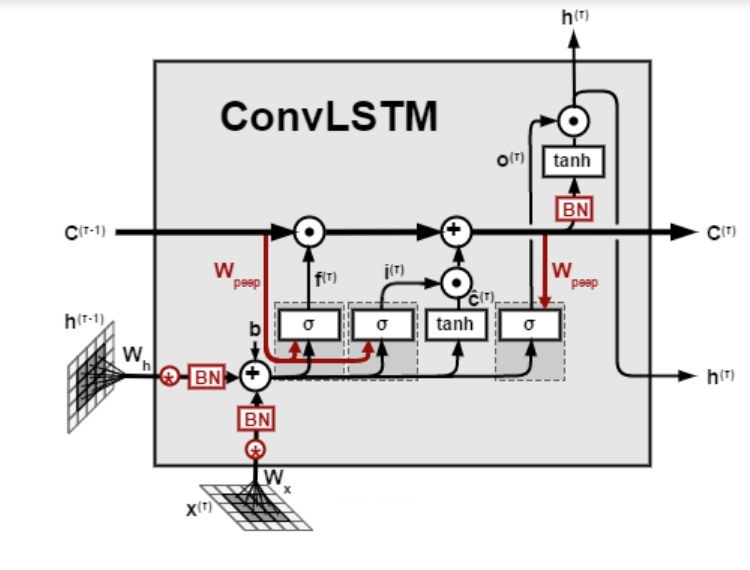
\includegraphics[width=0.7\textwidth]{Figures/convLSTM2D.jpg}
	\caption[ConvLSTM2D layer .]{ConvLSTM2D layer.}
	\label{convLSTM2D.jpg} 
    \end{figure}
Trong bước này, nhóm sẽ thực hiện phương pháp thứ 2 bằng cách sử dụng sự kết hợp của các ô ConvLSTM. Một ô ConvLSTM là một biến thể của mạng LSTM chứa các hoạt động tích chập trong mạng. Điều này là một LSTM với tích chập được nhúng trong kiến trúc, làm cho nó có khả năng xác định các đặc trưng không gian của dữ liệu trong khi vẫn giữ quan hệ thời gian.

Đối với phân loại video, phương pháp này hiệu quả trong việc nắm bắt mối quan hệ không gian trong các khung hình cá nhân và mối quan hệ thời gian qua các khung hình khác nhau. Kết quả của cấu trúc tích chập này, ConvLSTM có khả năng nhận đầu vào 3 chiều (chiều rộng, chiều cao, số kênh) trong khi LSTM đơn giản chỉ nhận đầu vào 1 chiều nên LSTM không tương thích để mô hình dữ liệu không gian-thời gian một cách độc lập.
Tương tự như lớp LSTM, nhưng các phép biến đổi đầu vào và các phép biến đổi hồi quy đều là tích chập.Lớp ConvLSTM2D thường được sử dụng để xử lý các chuỗi ảnh (video) 2 chiều .

ConvLSTM khác với LSTM ở chỗ nó kết hợp cả tính chất không gian (qua các bước tích chập) và tính chất thời gian (qua các bước LSTM), cho phép nó xử lý dữ liệu không gian-thời gian một cách hiệu quả. LSTM thông thường không có khả năng này vì nó chỉ xử lý dữ liệu theo một chiều thời gian.

Để hiểu rõ hơn về ConvLSTM2D hãy đọc bài báo \href{https://keras.io/api/layers/recurrent_layers/conv_lstm2d/}{Convolutional LSTM Network: A Machine Learning Approach for Precipitation Nowcasting} để hiểu hơn về kiến trúc này .

Lớp ConvLSTM2D cần 2 tham số chính:
\begin{itemize}
    \item Số bộ lọc (filters):Xác định số lượng bộ lọc để trích xuất các đặc điểm khác nhau từ ảnh .
    \item  Kích thước kernel (kernel size):Xác định kích thước của bộ lọc hình vuông sẽ được di chuyển trên ảnh để trích xuất các đặc điểm .
\end{itemize}

Đầu ra của lớp ConvLSTM2D là một tensor 4 chiều (batch\_size, timesteps, height, width), với :
\begin{itemize}
    \item batch\_size là số lượng mẫu trong mỗi lần tính toán.
    \item timesteps là số khung hình trong chuỗi ảnh.
    \item height và width là chiều cao và rộng của khung hình.
\end{itemize}


\subsubsection{Kiến trúc mô hình}
\begin{lstlisting}[style=codePython]
    model = Sequential()


    model.add(ConvLSTM2D(filters = 32, kernel_size = (3, 3), activation = 'tanh',data_format = "channels_last",
                         recurrent_dropout=0.2, return_sequences=True, input_shape = (SEQUENCE_LENGTH,IMAGE_HEIGH,IMAGE_WIDTH,3)))

    model.add(MaxPooling3D(pool_size=(1, 2, 2), padding='same', data_format='channels_last'))
    model.add(TimeDistributed(Dropout(0.2)))

    model.add(ConvLSTM2D(filters = 64, kernel_size = (3, 3), activation = 'tanh', data_format = "channels_last",
                         recurrent_dropout=0.2, return_sequences=True))

    model.add(MaxPooling3D(pool_size=(1, 2, 2), padding='same', data_format='channels_last'))
    model.add(TimeDistributed(Dropout(0.2)))

    model.add(ConvLSTM2D(filters = 64, kernel_size = (3, 3), activation = 'tanh', data_format = "channels_last",
                         recurrent_dropout=0.2, return_sequences=True))

    model.add(MaxPooling3D(pool_size=(1, 2, 2), padding='same', data_format='channels_last'))
    model.add(TimeDistributed(Dropout(0.2)))

    model.add(ConvLSTM2D(filters = 128, kernel_size = (3, 3), activation = 'tanh', data_format = "channels_last",
                         recurrent_dropout=0.2, return_sequences=True))

    model.add(MaxPooling3D(pool_size=(1, 2, 2), padding='same', data_format='channels_last'))

    model.add(Flatten())

    model.add(Dense(len(CLASSES_LIST), activation = "softmax"))

    model.summary()

\end{lstlisting}
Các tham số của convLSTM2D có thể hiểu như sau : 
\begin{itemize}
    \item input\_shape = (SEQUENCE\_LENGTH, IMAGE\_HEIGHT, IMAGE\_WIDTH, 3): Kích thước đầu vào, trong đó SEQUENCE\_LENGTH là độ dài chuỗi, IMAGE\_HEIGHT và IMAGE\_WIDTH là kích thước ảnh, và 3 là số kênh màu (RGB).
    \item filters = 32: Số lượng filter hoặc feature maps được áp dụng.
    \item kernel\_size = (3, 3): Kích thước của filter.
    \item activation = 'tanh': Hàm kích hoạt là tanh.
    \item data\_format = "channels\_last": Định dạng dữ liệu là "channels\_last" (chiều cuối cùng là kênh dữ liệu).
    \item recurrent\_dropout = 0.2: Tỷ lệ dropout cho các kết nối tái lặp trong LSTM.
    \item return\_sequences = True: Trả về chuỗi output thay vì chỉ output cuối cùng.
\end{itemize}
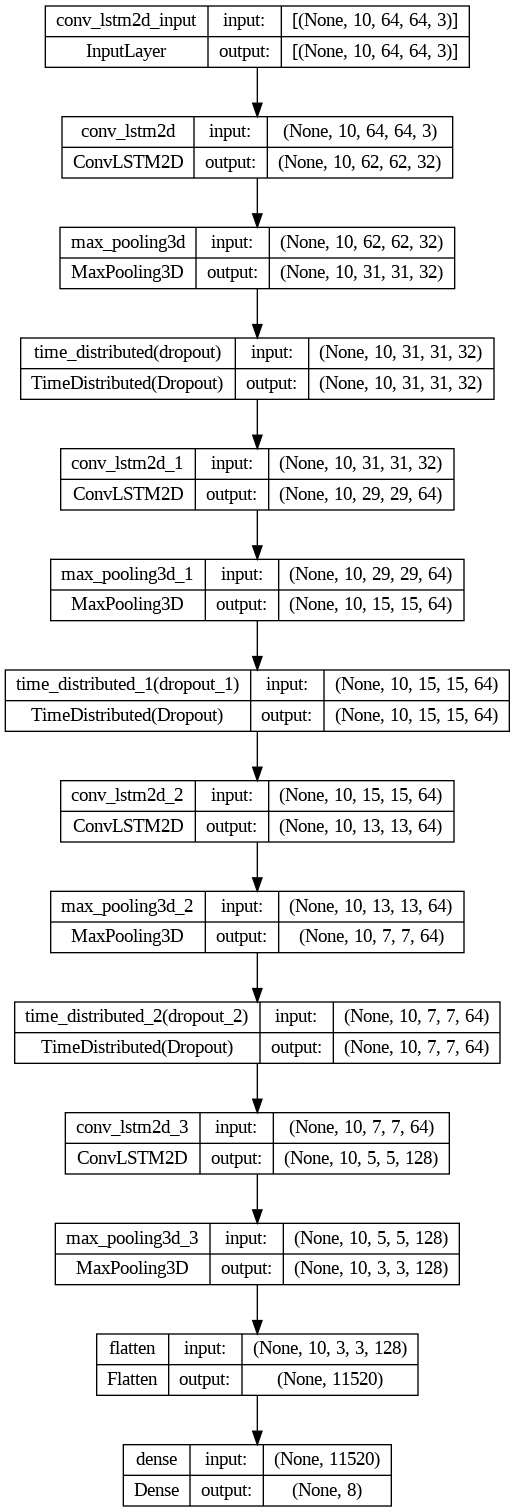
\includegraphics[width=0.5\textwidth]{Figures/model_conv.png}
\begin{figure}[ht!]
	\centering
	
	\caption[Model ConvLSTM2D.]{Model ConvLSTM2D.}
	\label{model_conv.png} 
    \end{figure}


Mô hình nhóm xây dựng để phân biệt 8 hành động , nên nhóm đã để Cuối cùng là 1 lớp kết nối đầy đủ với hàm kích hoạt softmax 
\subsection{Huấn luyện mô hình}
Bước tiếp theo nhóm thực hiện là thiết lập và huấn luyện mô hình 
\begin{lstlisting}[style=codePython]
early_stopping_callback = EarlyStopping(monitor = 'val_loss', patience = 10, mode = 'min', restore_best_weights = True)
convlstm_model.compile(loss = 'categorical_crossentropy', optimizer = 'Adam', metrics = ["accuracy"])

convlstm_model_training_history = convlstm_model.fit(x = X_train, y = y_train, epochs = 40,             
                                  batch_size=32,shuffle = True, validation_split = 0.2,callbacks,[early_stopping_callback])
\end{lstlisting}

Giải thích chi tiết : 
\begin{itemize}
    \item Early Stopping Callback:Sử dụng EarlyStopping callback để theo dõi 'val\_loss', chờ đợi 10 epochs trước khi dừng, theo chế độ 'min' (tối thiểu), và khôi phục trọng số tốt nhất khi kết thúc.
    \item Compile Model:Compile mô hình sử dụng hàm loss là 'categorical\_crossentropy', trình tối ưu hóa là 'Adam', và đánh giá theo chỉ số 'accuracy'.
    \item Training Model:Huấn luyện mô hình sử dụng dữ liệu đầu vào X\_train và nhãn y\_train, với 40 epochs, batch size là 32, xáo trộn dữ liệu, phân chia validation set là 20\%, và sử dụng callbacks bao gồm early\_stopping\_callback.
\end{itemize}

\subsubsection{Đánh giá mô hình}
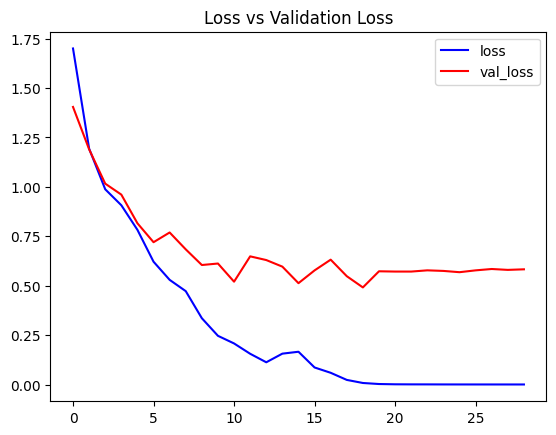
\includegraphics[width=0.5\textwidth]{Figures/loss_conv.png} \&
		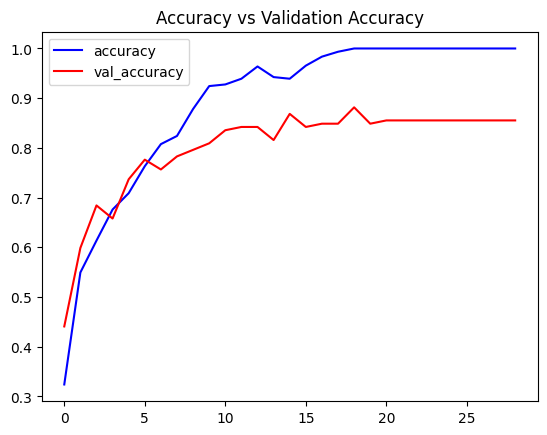
\includegraphics[width=0.5\textwidth]{Figures/val_conv.png}
\begin{figure}[h!] 
	\begin{tabular}{cc}
		\centering
		 
	\end{tabular}
	\caption[Model Accuracy và Model Loss.]{Model Accuracy và Model Loss.}
	\label{fig:modelloss_and_Model Accuracy}
\end{figure}

Đồ thị ACC,  độ chính xác (Accuracy) lên đến 98\% và bắt đầu ổn định khi epoch = 30,  cho cả tập dữ liệu huấn luyện và 86\% tập test, đồ thị Loss của cũng cho thấy sau mức này, Loss của cả tập train và validation. Kết quả cho thấy mô hình có độ phù hợp tốt và không bị quá khớp (over-fitting).

\begin{itemize}
    \item Đánh giá hiệu suất mô hình:
    	
    	\begin{figure}[h!]
    		\centering
    		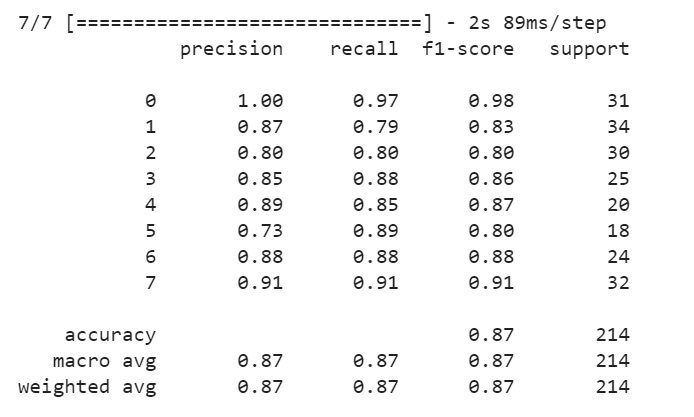
\includegraphics[width=0.7\textwidth]{Figures/evaluate_conv.PNG}
    		\caption[Đánh giá hiệu suất mô hình.]{Đánh giá hiệu suất mô hình.}
    		\label{fig:ac} 
    	\end{figure}
	
	\item Confusion Matrix:
	
	\begin{figure}[h!]
		\centering
		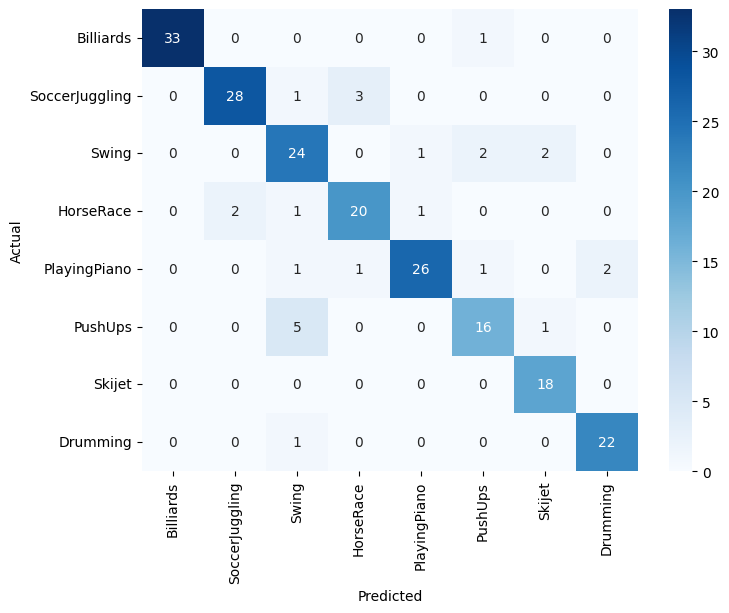
\includegraphics[width=0.6\textwidth]{Figures/conv_confusion.png}
		\caption[Confusion Matrix.]{Confusion Matrix.}
		\label{fig:conv_confusion.png} 
	\end{figure}
\end{itemize}

\subsection{Xây dựng mô hình \href{https://arxiv.org/abs/1411.4389?source=post_page---------------------------}{LRCN}}
    \begin{figure}[h!]
	\centering
	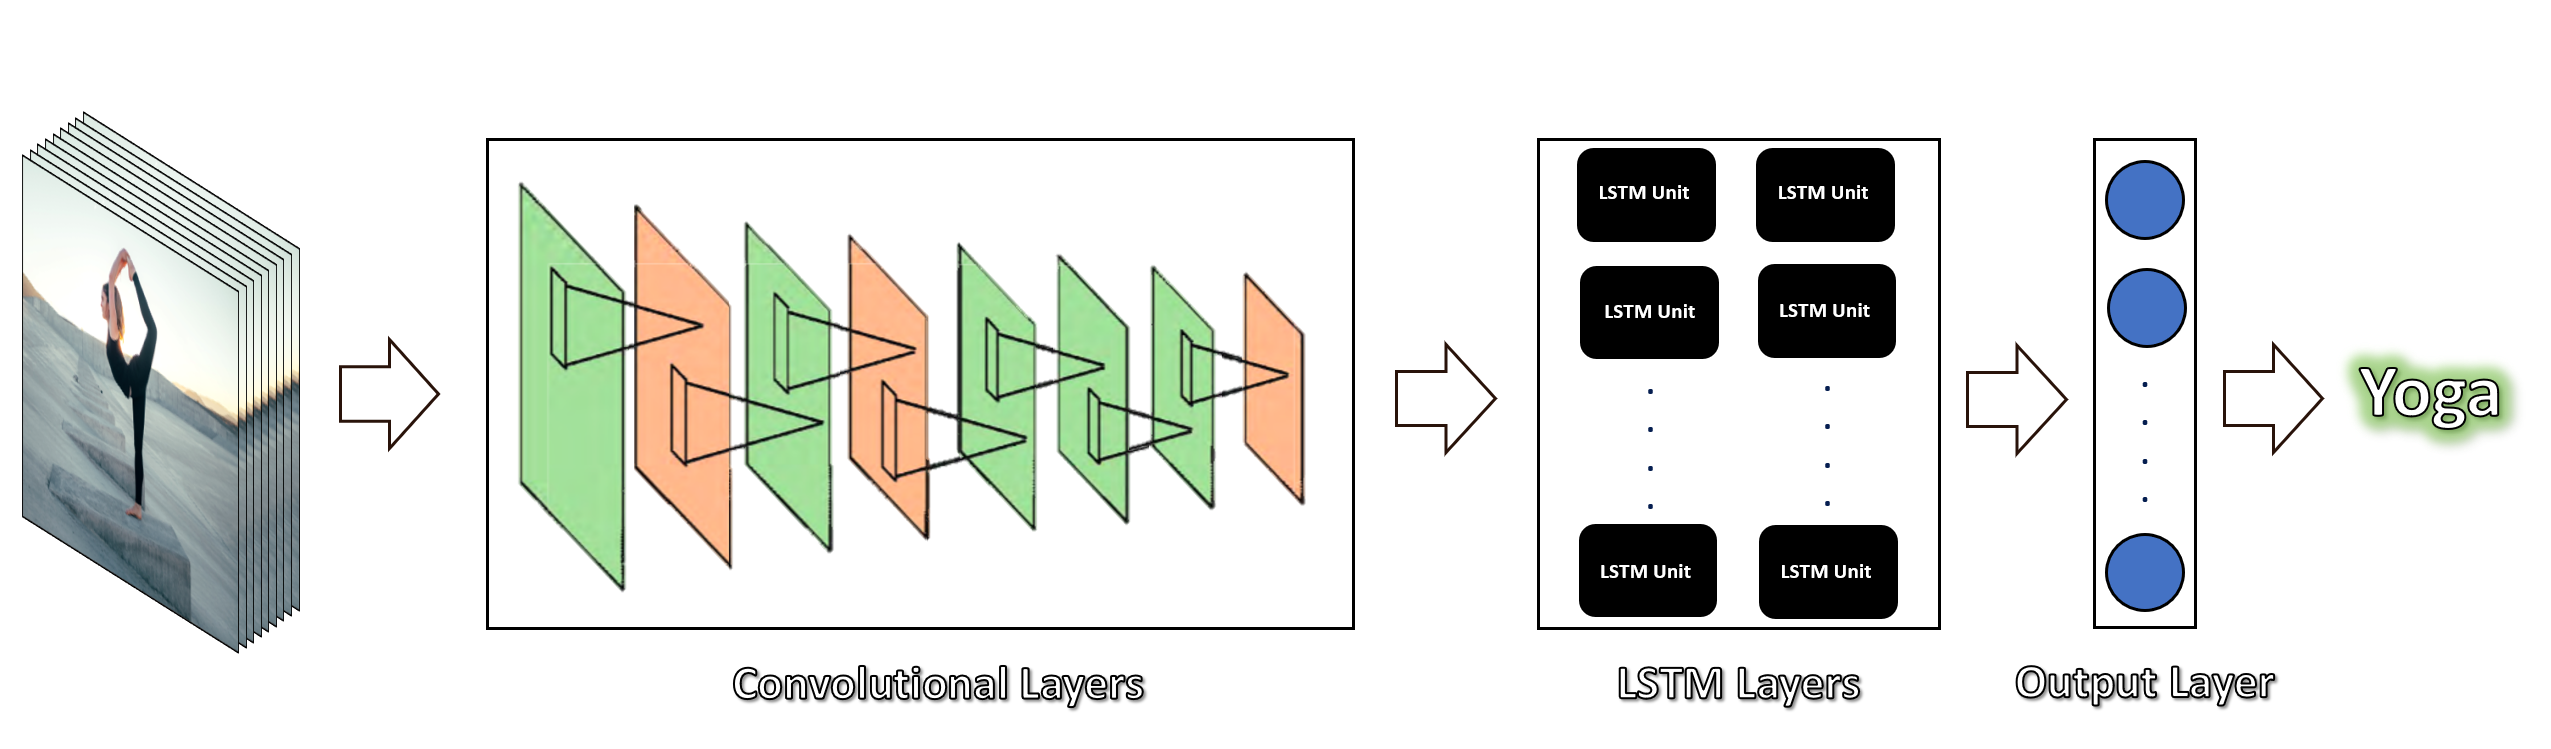
\includegraphics[width=0.7\textwidth]{Figures/LRCN.png}
	\caption[LRCN model .]{LRCN model.}
	\label{LRCN.png} 
    \end{figure}
Trong bước này, nhóm sẽ thực hiện phương pháp thứ 3 xây dựng mô hình LRCN ( Long-Term Recurrent Convolutional Network)

Mô hình LRCN (Long-Term Recurrent Convolutional Network) là một mô hình học sâu được sử dụng cho các tác vụ xử lý dữ liệu hình ảnh tuần tự, chẳng hạn như phân loại video, nhận dạng hành động và chú thích hình ảnh.

Mô hình LRCN là một mô hình kết hợp các lớp Convolutional và LSTM trong một mô hình duy nhất.Mô hình LRCN bao gồm hai thành phần chính:
\begin{itemize}
    \item Các lớp Convolutional trích xuất các đặc trưng không gian từ từng khung hình.
    \item Các đặc trưng này được đưa trực tiếp vào các lớp LSTM tại từng bước thời gian để mô hình chuỗi thời gian.
\end{itemize}
Cách tiếp cận này cho phép mô hình học trực tiếp các đặc trưng không gian thời gian trong quá trình huấn luyện end-to-end, dẫn đến một mô hình mạnh mẽ hơn.
Cụ thể, mô hình LRCN hoạt động như sau:
\begin{itemize}
    \item Dữ liệu đầu vào (các sequence hình ảnh) được đưa vào các lớp convolution 2D. Các lớp convolution 2D sẽ trích xuất các đặc trưng không gian từ từng frame trong sequence.
    \item Các đặc trưng không gian từ các frames được kết hợp lại và đưa vào lớp LSTM. Lớp LSTM sẽ xử lý thông tin thời gian giữa các frames.
    \item Lớp LSTM sẽ tạo ra một vector biểu diễn cho toàn bộ sequence.
    \item Vector biểu diễn này được đưa vào một lớp phân loại để dự đoán kết quả của tác vụ.
\end{itemize}

Mô hình LRCN có một số ưu điểm sau:
\begin{itemize}
    \item Có thể trích xuất các đặc trưng không gian và thời gian từ dữ liệu hình ảnh tuần tự.
    \item Có thể nắm bắt các mối quan hệ dài hạn giữa các frames trong một sequence.
    \item Có thể huấn luyện end-to-end, đơn giản hóa quá trình huấn luyện.
\end{itemize}

Tuy nhiên, mô hình LRCN cũng có một số nhược điểm sau:
\begin{itemize}
    \item Có thể gặp khó khăn trong việc nắm bắt các mối quan hệ phức tạp giữa các đặc trưng không gian và thời gian.
    \item Có thể khó huấn luyện.

\end{itemize}

Mô hình LRCN đã được áp dụng thành công cho nhiều tác vụ xử lý dữ liệu hình ảnh tuần tự, chẳng hạn như:
\begin{itemize}
    \item Phân loại video
    \item Nhận dạng hành động
    \item Chú thích hình ảnh
    \item Theo dõi đối tượng
\end{itemize}

Dưới đây là một số ví dụ về ứng dụng của mô hình LRCN:
\begin{itemize}
    \item Phân loại video thành các loại khác nhau, chẳng hạn như thể thao, tin tức, giải trí, v.v.
    \item Nhận dạng các hành động của con người trong video, chẳng hạn như đi bộ, chạy, nhảy, v.v.
    \item Chú thích hình ảnh bằng văn bản, chẳng hạn như mô tả nội dung của hình ảnh.
    \item Theo dõi đối tượng trong video, chẳng hạn như xác định vị trí của một người trong video.
\end{itemize}



\subsubsection{Kiến trúc mô hình}
\begin{lstlisting}[style=codePython]
def create_LRCN_model():


    model = Sequential()


    model.add(TimeDistributed(Conv2D(16, (3, 3), padding='same',activation = 'relu'),
                              input_shape = (SEQUENCE_LENGTH, IMAGE_HEIGHT, IMAGE_WIDTH, 3)))

    model.add(TimeDistributed(MaxPooling2D((4, 4))))
    model.add(TimeDistributed(Dropout(0.25)))

    model.add(TimeDistributed(Conv2D(32, (3, 3), padding='same',activation = 'relu')))
    model.add(TimeDistributed(MaxPooling2D((4, 4))))
    model.add(TimeDistributed(Dropout(0.25)))

    model.add(TimeDistributed(Conv2D(64, (3, 3), padding='same',activation = 'relu')))
    model.add(TimeDistributed(MaxPooling2D((2, 2))))
    model.add(TimeDistributed(Dropout(0.25)))

    model.add(TimeDistributed(Conv2D(64, (3, 3), padding='same',activation = 'relu')))
    model.add(TimeDistributed(MaxPooling2D((2, 2))))
    #model.add(TimeDistributed(Dropout(0.25)))

    model.add(TimeDistributed(Flatten()))

    model.add(LSTM(32))

    model.add(Dense(len(CLASSES_LIST), activation = 'softmax'))


    model.summary()


    return model

\end{lstlisting}
Lớp TimeDistributed(Conv2D) thực hiện các bước sau : 
\begin{itemize}
    \item TimeDistributed: Đảm bảo lớp Conv2D được áp dụng cho từng frame riêng lẻ trong chuỗi hình ảnh.
    \item Conv2D(16, (3, 3), padding='same', activation='relu'): Tạo một lớp convolutional 2D với các thông số sau:
    \item input\_shape = (SEQUENCE\_LENGTH, IMAGE\_HEIGHT, IMAGE\_WIDTH, 3): Kích thước đầu vào, trong đó SEQUENCE\_LENGTH là độ dài chuỗi, IMAGE\_HEIGHT và IMAGE\_WIDTH là kích thước ảnh, và 3 là số kênh màu (RGB).
\end{itemize}
\newpage
\begin{figure}[h!]
	\centering
	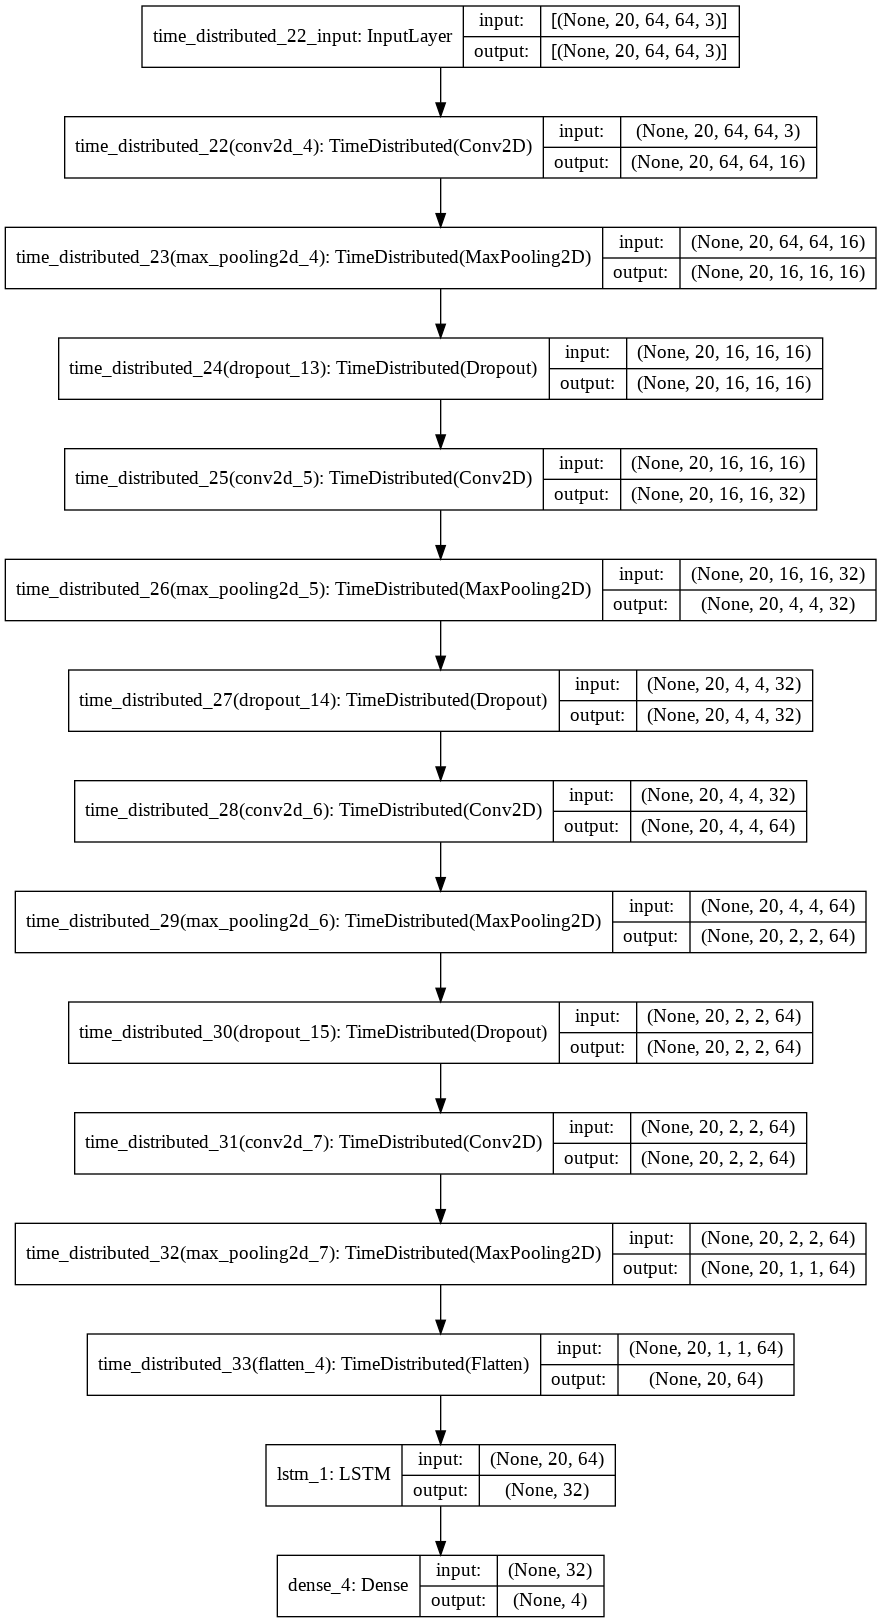
\includegraphics[width=0.7\textwidth]{Figures/model_lrcn.png}
	\caption[Kiến trúc model LRCN.]{Kiến trúc model LRCN.}
	\label{model_lrcn.png} 
    \end{figure}
\newpage
Mô hình nhóm xây dựng để phân biệt 8 hành động , nên nhóm đã để Cuối cùng là 1 lớp kết nối đầy đủ với hàm kích hoạt softmax 

Bước tiếp theo nhóm thực hiện là thiết lập và huấn luyện mô hình  áp dụng giống như cách làm với mô hình sử dụng convLSTM2D

\subsubsection{Đánh giá mô hình}
		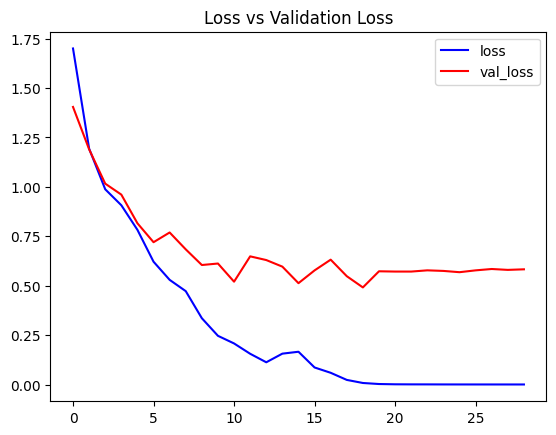
\includegraphics[width=0.5\textwidth]{Figures/loss_conv.png} \&
		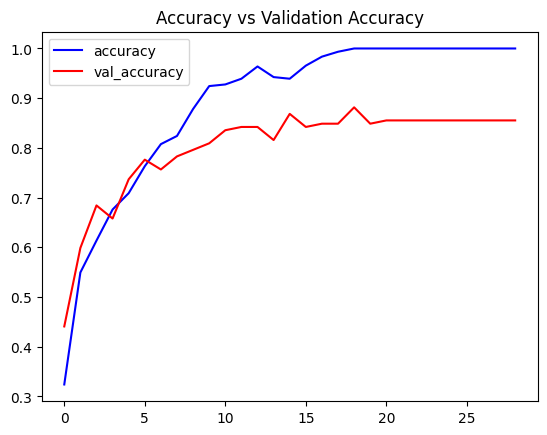
\includegraphics[width=0.5\textwidth]{Figures/val_conv.png}
\begin{figure}[h!] 
	\begin{tabular}{cc}
		\centering
    
	\end{tabular}
	\caption[Model Accuracy và Model Loss.]{Model Accuracy và Model Loss.}
	\label{fig:modelloss_and_Model Accuracy}
\end{figure}

Đồ thị ACC,  độ chính xác (Accuracy) lên đến 97\% và bắt đầu ổn định khi epoch = 20,  cho cả tập dữ liệu huấn luyện và và 90\% tập test, đồ thị Loss của cũng cho thấy sau mức này, Loss của cả tập train và validation. Kết quả cho thấy mô hình có độ phù hợp tốt và không bị quá khớp (over-fitting).
\newpage
\begin{itemize}
	\item Đánh giá hiệu suất mô hình:
 
	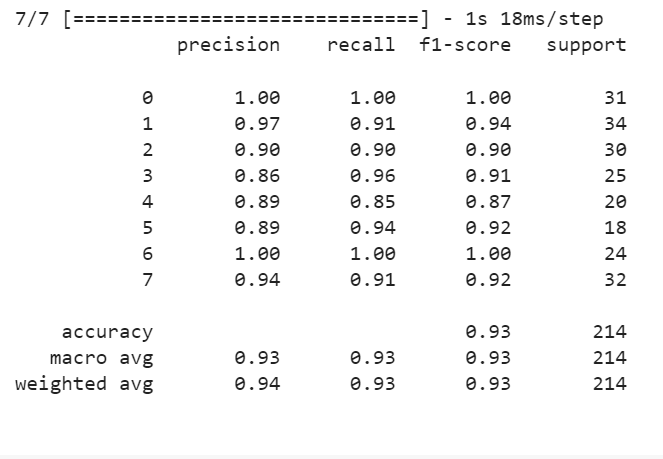
\includegraphics[width=0.7\textwidth]{Figures/evaluate_lrcn.PNG}
	\begin{figure}[h!] 
	\begin{tabular}{cc}
		\centering
	\end{tabular}
	\caption[Đánh giá hiệu suất mô hình.]{Đánh giá hiệu suất mô hình.}
	\label{fig:modelloss_and_Model Accuracy}
\end{figure}
	\item Confusion Matrix:
	
	\begin{figure}[h!]
		\centering
		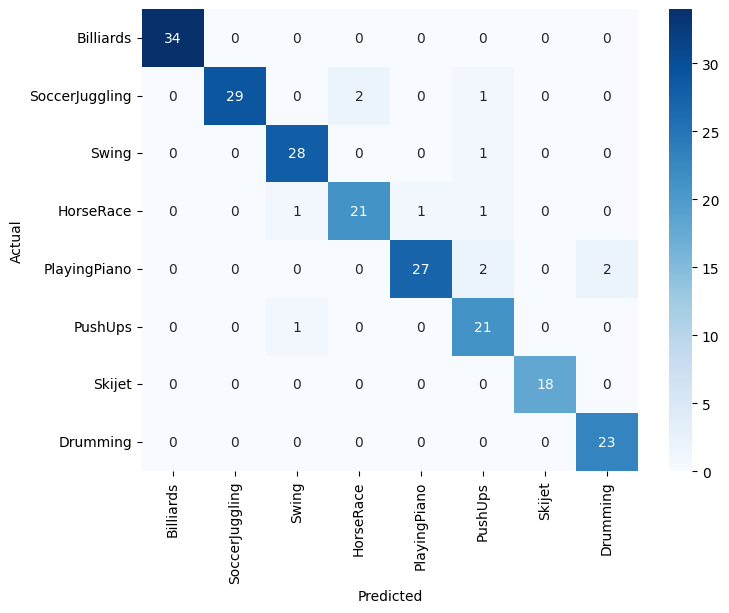
\includegraphics[width=0.6\textwidth]{Figures/lstm_confusion.png}
		\caption[Confusion Matrix.]{Confusion Matrix.}
		\label{fig:lstm_confusion} 
	\end{figure}
\end{itemize}
\subsection{Thử nghiệm với video download từ youtube}
Bước 1 : Download video từ youtube : 
Hàm download\_youtube\_video có nhiệm vụ download video từ link youtube .
\begin{lstlisting}[style=codePython]
def download_youtube_video(url, output_path):
    try:
        youtube = pytube.YouTube(url)
        video = youtube.streams.get_highest_resolution()
        title = video.title
        output_file_path = f"{output_path}/{title}.mp4"
        video.download(output_path)
        return title
    except Exception as e:
        print("Error: ", str(e))
        return None
\end{lstlisting}

Bước 2 : Viết hàm dự đoán hành động trong video 

\begin{lstlisting}[style=codePython]
def predict_on_video(video_file_path, output_file_path, SEQUENCE_LENGTH):


    video_reader = cv2.VideoCapture(video_file_path)

    original_video_width = int(video_reader.get(cv2.CAP_PROP_FRAME_WIDTH))
    original_video_height = int(video_reader.get(cv2.CAP_PROP_FRAME_HEIGHT))

    video_writer = cv2.VideoWriter(output_file_path, cv2.VideoWriter_fourcc('M', 'P', '4', 'V'),
                                   video_reader.get(cv2.CAP_PROP_FPS), (original_video_width, original_video_height))

    frames_queue = deque(maxlen = SEQUENCE_LENGTH)

    predicted_class_name = ''

    while video_reader.isOpened():

        _, frame = video_reader.read()

        if not _:
            break

        resized_frame = cv2.resize(frame, (IMAGE_HEIGHT, IMAGE_WIDTH))

        normalized_frame = resized_frame / 255

        frames_queue.append(normalized_frame)

        if len(frames_queue) == SEQUENCE_LENGTH:

            predicted_labels_probabilities = convlstm_model.predict(np.expand_dims(frames_queue, axis = 0))[0]

            predicted_label = np.argmax(predicted_labels_probabilities)

            predicted_class_name = CLASSES_LIST[predicted_label]

        cv2.putText(frame, predicted_class_name, (10, 30), cv2.FONT_HERSHEY_SIMPLEX, 1, (0, 255, 0), 2)

        video_writer.write(frame)

    video_reader.release()
    video_writer.release()
\end{lstlisting}


Trong đoạn code trên cần chú ý  : 
\begin{itemize}
    \item frames\_queue = deque(maxlen=SEQUENCE\_LENGTH): Tạo một hàng đợi (queue) để lưu trữ các khung hình, giới hạn số lượng khung hình tối đa là SEQUENCE\_LENGTH. 
\end{itemize}
